\section{\secclassifygraphs}
\label{sec_classify_graphs}

A common theme across the sciences is to classify objects of a particular type.  For example, how might we classify all trees with seven vertices?  Since there are only finitely many, we can create a list of trees having seven vertices so that any tree with seven vertices is isomorphic to a tree on our list and no two trees on our list are isomorphic.  
We begin by discussing how to show that two graphs are not isomorphic.

%%%%%%%%%%%%%%%%%%%%

\newcommand{\subnonisograph}{Nonisomorphic Graphs}
\subsection{\subnonisograph}
\label{sub_nonisomorphic_graphs}

Here is a not terribly useful definition of nonisomorphic graphs.

\begin{defn}[Nonisomorphic]
\label{defn_nonism}
    Two graphs $G$ and $H$ are \vocab{nonisomorphic}, denoted $G \ncong H$, if they are not isomorphic. That is, if it is impossible to label the vertices of $G$ and the vertices of $H$ in such a way that $G$ and $H$ have the same vertices and the same edges.    
\end{defn}

This definition is not useful in writing proofs because it is subtle to prove that something is impossible.  We might not find a way to label the vertices that shows that two graphs are isomorphic, but that does not prove that there is no labeling.  We might not be able to visualize how one graph can be transformed into the other, but that does not mean that there is no way to do so. Let's look at an example.

\begin{exam}[Showing $G_1$ and $G_3$ are nonisomorphic]
\label{exam_not_ism}
    Although they share many common properties, the graphs $G_1$ and $G_3$ drawn in \Cref{fig_G1G2G3} are not isomorphic. Prove it.
        \begin{soln}
            Let's start with the labeling of $G_1$ from \Cref{fig_G1G2_labeled}.  The only degree 3 vertex in $G_1$ is labeled $c$.  That means $c$ is the only vertex that appears in exactly three edges.  The graph $G_3$ has one degree 3 vertex, and if we want to produce the same edge list as $G_1$, that vertex needs to be labeled $c$ to match, as shown in \Cref{fig_failed_labeling}.  
            
        \begin{figure}[hbtp]
            \centering
            %Used in \Cref{sec_graph_ism}.

\begin{tikzpicture}
[scale =.5]
\GraphInit[vstyle=Welsh]
\SetGraphUnit{1.6}
%\SetVertexNoLabel
\node at (4,4) {$G_1$};
\Vertex[LabelOut,Lpos=90,x=0,y=2]{$a$}
\Vertex[LabelOut,Lpos= 90,x=2,y=2]{$b$}
\Vertex[LabelOut,Lpos= 90,x=4,y=2]{$c$}
\Vertex[LabelOut,Lpos= 90,x=6,y=2]{$d$}
\Vertex[LabelOut,Lpos= 90,x=8,y=2]{$e$}
\Vertex[LabelOut,Lpos= 0,x=4,y=0]{$x$}
\Edges($a$, $b$, $c$, $d$, $e$)
\Edges($c$,$x$)
\end{tikzpicture}
\hspace{1in} %%%%%
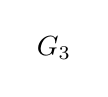
\begin{tikzpicture}
[scale =.5]
\GraphInit[vstyle=Welsh]
\SetGraphUnit{2}
%\SetVertexNoLabel
\node at (4,4) {$G_3$};
\Vertex[LabelOut,Lpos=90,x=0,y=2]{$?$}
\Vertex[LabelOut,Lpos= 90,x=2,y=2]{$c$}
\Vertex[NoLabel,x=4,y=2]{$z$}
\Vertex[NoLabel,x=6,y=2]{$d$}
\Vertex[NoLabel,x=8,y=2]{$e$}
\Vertex[LabelOut,Lpos= 0,x=2,y=0]{$x$}
\Edges($?$, $c$, $z$, $d$, $e$)
\Edges($c$,$x$)
\end{tikzpicture}
            \caption{Trying to label $G_3$ to match $G_1$ (and failing).}
            \label{fig_failed_labeling}
        \end{figure}             
            Next, in $G_1$, the vertex $c$ has exactly one neighbor with degree one, and it is labeled $x$.
            But in $G_3$, the vertex $c$ has two neighbors with degree one.  If we label one of those neighbors $x$, the other cannot be labeled (?). We are stuck.  There is no common labeling.  Therefore, $G$ and $K$ are not isomorphic.

            Notice that we have identified a property that distinguishes $G_1$ from $G_3$, namely $G_1$ has exactly one vertex with degree three and that vertex has exactly one neighbor with degree one, but $G_3$ does not have that property. This observation gives us a shorter proof that $G_1$ and $G_3$ are not isomorphic. After all, if they were the same graph, then they would have shared all graph-theoretic properties.
        \end{soln}
\end{exam} 

We can make the type of argument we used in \Cref{exam_not_ism} more formal.  We start with another definition.

\begin{defn}[Graph invariant]
\label{defn_graph_invariant}
    A \vocab{graph invariant} is a property $\mathcal{P}$ that satisfies 
        \begin{center} 
            ($\star$) If a graph $G$ has the property $\mathcal{P}$ and $G \cong H$, then $H$ also has the property $\mathcal{P}$.  
        \end{center}
    For example, ``having exactly one degree three vertex'' is a graph invariant. 
\end{defn}

\begin{exam}[Examples of graph invariants]
\label{exam_graph_invariants}
  List some examples of specific graph invariants.
     \begin{soln}
         Here are some arbitrary examples.  
             \begin{bull}
                \item Having exactly ten vertices.
                \item Having exactly six edges.
                \item Having exactly three vertices of degree four.
                \item Having a vertex of degree four that is adjacent to two vertices of degree one.
                \item Having the degree sequence $3,3,2,2,2,2$.
                \item Containing a 3-cycle.
                \item Not containing any 4-cycles.
                \item Containing two 4-cycles.
                \item Being acyclic.
                \item Containing a subgraph isomorphic to $K_4$.
                \item Having a path of length eight.
                \item Being connected.
                \item Having chromatic number three.
                \item and so on.
            \end{bull}
        Officially, we should prove that each of these properties is a graph invariant. Some properties that are \emph{not} graph invariants are ``is drawn as a 5-cycle plus edges'' or ``has adjacent vertices labeled $a$ and $b$''.  More generally, any property that refers to how a graph is drawn or labeled is not a graph invariant.
    \end{soln}
\end{exam}

We can use graph invariants to prove that two graphs are not isomorphic.

\begin{rem}[Using graph invariants to prove that two graphs are not isomorphic]
\label{rem_show_not_ism}
    If two graphs are isomorphic, then they are the same graph, and therefore they must agree on all graph invariants. Equivalently\footnote{The statement $\star\star$ is the contrapositive of $\star$.  We will prove in \Cref{sec_converse_cp} that a statement and its contrapositive are logically equivalent.}, for a graph invariant $\mathcal{P}$,
        \begin{center} 
            ($\star\star$) If a graph $G$ has the property $\mathcal{P}$ but the graph $H$ does not have the property $\mathcal{P}$, then $G \ncong H$.  
        \end{center}
    Therefore, to prove that graphs $G$ and $H$ are not isomorphic, we can find an invariant that $G$ has but $H$ does not or vice versa.
\end{rem}

Let's look at an example.

\begin{exam}[Use a graph invariant to show not isomorphic]
\label{exam_use_graph_invariant_show_nonism}
~
        \begin{apart}
            \item \label{part_nonism_order4} Show that the graphs $D_1$ and $D_2$ drawn in \Cref{fig_notism_C4} are not isomorphic by finding a distinguishing graph invariant.
                \begin{figure}[hbtp]
                    \centering
                    %Used in \Cref{sec_graph_ism}.

\begin{tikzpicture}
[scale =.35]
\GraphInit[vstyle=Welsh]
\SetGraphUnit{1.6}
\SetVertexNoLabel
\node at (-2,3) {$D_1$};
\Vertex[LabelOut,Lpos=90,x=0,y=3]{$A$}
\Vertex[LabelOut,Lpos= 90,x=3,y=3]{$B$}
\Vertex[LabelOut,Lpos=-90,x=3,y=0]{$C$}
\Vertex[LabelOut,Lpos=-90,x=0,y=0]{$D$}
\Edges($A$, $B$, $D$, $A$)
\Edges($B$,$C$)
\end{tikzpicture}
\hspace{1 in} %%%%%
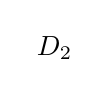
\begin{tikzpicture}
[scale =.35]
\GraphInit[vstyle=Welsh]
\SetGraphUnit{1.6}
\SetVertexNoLabel
\node at (-2,3) {$D_2$};
\Vertex[LabelOut,Lpos=90,x=0,y=3]{$A$}
\Vertex[LabelOut,Lpos= 90,x=3,y=3]{$B$}
\Vertex[LabelOut,Lpos=-90,x=3,y=0]{$C$}
\Vertex[LabelOut,Lpos=-90,x=0,y=0]{$D$}
\Edges($A$, $B$, $C$, $D$, $A$)
\end{tikzpicture}

                    \caption{Nonisomorphic graphs from \Cref{exam_use_graph_invariant_show_nonism} (\ref{part_nonism_order4}).}
                    \label{fig_notism_C4}
                \end{figure}
                \begin{soln}
                    One reason $D_1$ and $D_2$ are nonisomorphic is that $D_1$ has a vertex of degree one and $D_2$ does not.  Another reason is that they have different degree sequences:  $3,2,2,1$ for $D_1$ versus $2,2,2,2$ for $D_2$.  Yet another reason is $D_2$ contains a 4-cycle but $D_1$ does not.  And so on. Only one distinguishing graph invariant is needed. For any of these reasons, $D_1 \ncong D_2$.
                \end{soln}
            \item Show that the graphs $E_1$ and $E_2$ drawn in \Cref{fig_notism_Ham8} are not isomorphic by finding a distinguishing graph invariant.
                \begin{figure}[hbtp]
                    \centering
                    %Used in \Cref{sec_graph_ism}.

\begin{tikzpicture}
[scale =.5, auto=left]
\GraphInit[vstyle=Welsh]
\SetGraphUnit{1.6}
\SetVertexNoLabel
\node at (-2.5,2.5) {$E_1$};
\Vertices{circle}{$c$,$b$,$a$,$h$,$g$,$f$,$e$,$d$}
\Edges($a$,$b$,$c$,$d$,$e$,$f$,$g$,$h$,$a$)
\Edges($a$,$e$)
\end{tikzpicture}
\hspace{1in} %%%%%
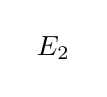
\begin{tikzpicture}
[scale =.5, auto=left]
\GraphInit[vstyle=Welsh]
\SetGraphUnit{1.6}
\SetVertexNoLabel
\node at (-2.5,2.5) {$E_2$};
\Vertices{circle}{$c$,$b$,$a$,$h$,$g$,$f$,$e$,$d$}
\Edges($a$,$b$,$c$,$d$,$e$,$f$,$g$,$h$,$a$)
\Edges($a$,$d$)
\end{tikzpicture}

                    \caption{The graphs $E_1$ and $E_2$ are not isomorphic.}
                    \label{fig_notism_Ham8}
                \end{figure}
                \begin{soln}              
                    One reason $E_1$ and $E_2$ are nonisomorphic is that $E_1$ contains two 5-cycles and $E_2$ does not contain any 5-cycles.  Another reason is that $E_2$ can be 2-colored but $E_1$ cannot, as shown in \Cref{fig_notism_Ham8_bipartite}. 
                        \begin{figure}[hbtp]
                            \centering
                            %Used in \Cref{sec_graph_ism}.

\begin{tikzpicture}
[scale =.5, auto=left]
\GraphInit[vstyle=Welsh]
\SetGraphUnit{1.6}
\SetVertexNoLabel
\node at (-2.5,2.5) {$E_1$};
\Vertices{circle}{$c$,$b$,$a$,$h$,$g$,$f$,$e$,$d$}
\Edges($a$,$b$,$c$,$d$,$e$,$f$,$g$,$h$,$a$)
\Edges($a$,$e$)
\AddVertexColor{black}{$a$, $c$, $g$}
\AddVertexColor{gray}{$e$}
\end{tikzpicture}
\hspace{1in} %%%%%
\begin{tikzpicture}
[scale =.5, auto=left]
\GraphInit[vstyle=Welsh]
\SetGraphUnit{1.6}
\SetVertexNoLabel
\node at (-2.5,2.5) {$E_2$};
\Vertices{circle}{$c$,$b$,$a$,$h$,$g$,$f$,$e$,$d$}
\Edges($a$,$b$,$c$,$d$,$e$,$f$,$g$,$h$,$a$)
\Edges($a$,$d$)
\AddVertexColor{black}{$a$, $c$, $e$, $g$}
\end{tikzpicture}

                            \caption{The graph $E_2$ can be 2-colored but the graph $E_1$ cannot.}
                            \label{fig_notism_Ham8_bipartite}
                        \end{figure}                     
                    Note that any 2-coloring of $E_1$ would have to alternate around the 8-cycle but then the opposite end of the chord would have to be a third color. A different, quite complicated reason why $E_1$ and $E_2$ are nonisomorphic is that in $E_2$ there is a pair of adjacent degree two vertices each of which has a degree three neighbor (the black vertex and white vertex to the right of the chord edge), but in $E_1$ no pair of adjacent degree two both have degree three neighbors. For any of these reasons, $E_1 \ncong E_2$.
                \end{soln}
        \end{apart}
\end{exam}

Your turn to practice showing graphs are not isomorphic and deciding whether or not two graphs are isomorphic.

\begin{act}[Show two graphs are not isomorphic]
\label{act_show_nonism_or_decide}
~
    \begin{actpart}
        \item \label{part_act_common_ppty} Check that the graphs drawn in \Cref{fig_nonism_graphs_act} have the same number of vertices, the same number of edges, and the same degree sequence and find a 4-cycle in each graph.  
            \begin{figure}[hbtp]
                \centering
                %Used in \Cref{sec_graph_ism}.

\begin{tikzpicture}
[scale =.35]
\GraphInit[vstyle=Welsh]
\SetGraphUnit{1.6}
\SetVertexNoLabel
\Vertex[LabelOut,Lpos=90,x=0,y=3]{$a_1$}
\Vertex[LabelOut,Lpos=90,x=3,y=3]{$b_1$}
\Vertex[LabelOut,Lpos=90,x=6,y=3]{$c_1$}
\Vertex[LabelOut,Lpos=90,x=9,y=3]{$d_1$}
\Vertex[LabelOut,Lpos=-90,x=0,y=0]{$a_2$}
\Vertex[LabelOut,Lpos=-90,x=3,y=0]{$b_2$}
\Vertex[LabelOut,Lpos=-90,x=6,y=0]{$c_2$}
\Vertex[LabelOut,Lpos=-90,x=9,y=0]{$d_2$}
\Edges($a_1$, $b_1$, $c_1$, $d_1$)
\Edges($a_2$, $b_2$, $c_2$, $d_2$)
\Edges($a_1$,$a_2$)
\Edges($b_1$,$c_2$)
\Edges($b_2$,$c_1$)
\end{tikzpicture}
\hspace{1 in} %%%%%
\begin{tikzpicture}
[scale =.35]
\GraphInit[vstyle=Welsh]
\SetGraphUnit{1.6}
\SetVertexNoLabel
\Vertex[LabelOut,Lpos=90,x=0,y=3]{$a_1$}
\Vertex[LabelOut,Lpos=90,x=3,y=3]{$b_1$}
\Vertex[LabelOut,Lpos=90,x=6,y=3]{$c_1$}
\Vertex[LabelOut,Lpos=90,x=9,y=3]{$d_1$}
\Vertex[LabelOut,Lpos=-90,x=0,y=0]{$a_2$}
\Vertex[LabelOut,Lpos=-90,x=3,y=0]{$b_2$}
\Vertex[LabelOut,Lpos=-90,x=6,y=0]{$c_2$}
\Vertex[LabelOut,Lpos=-90,x=9,y=0]{$d_2$}
\Edges($a_1$, $b_1$, $c_1$, $d_1$)
\Edges($a_2$, $b_2$, $c_2$, $d_2$)
\Edges($a_1$,$a_2$)
\Edges($b_1$,$b_2$)
\Edges($c_2$,$c_1$)
\end{tikzpicture}

                \caption{Nonisomorphic graphs for \Cref{act_show_nonism_or_decide} (\ref{part_act_common_ppty}) and (\ref{part_act_nonism}).}
                \label{fig_nonism_graphs_act}
            \end{figure}
        \item \label{part_act_nonism} Show that the graphs drawn in \Cref{fig_nonism_graphs_act} are nonisomorphic by finding a graph invariant that distinguishes the two graphs.
        \item \label{part_act_nonism_trees} Show the trees drawn in \Cref{fig_nonism_trees_act} are nonisomorphic by finding a graph invariant that distinguishes the two graphs.
            \begin{figure}[hbtp]
                \centering
                %Used in \Cref{sec_graph_ism}.

\begin{tikzpicture}
[scale =.4]
\GraphInit[vstyle=Welsh]
\SetGraphUnit{2}
\SetVertexNoLabel
\Vertex[LabelOut,Lpos=90,x=0,y=0]{$a$}
\Vertex[LabelOut,Lpos= 90,x=2,y=0]{$b$}
\Vertex[LabelOut,Lpos= 90,x=4,y=0]{$c$}
\Vertex[LabelOut,Lpos= 90,x=6,y=0]{$d$}
\Vertex[LabelOut,Lpos= 90,x=8,y=0]{$e$}
\Vertex[LabelOut,Lpos= 90,x=10,y=0]{$f$}
\Vertex[LabelOut,Lpos= 90,x=4,y=-2]{$r$}
\Vertex[LabelOut,Lpos= 90,x=8,y=-2]{$s$}
\Edges($a$, $b$, $c$, $d$, $e$,$f$)
\Edges($c$,$r$)
\Edges($e$,$s$)
\end{tikzpicture}
\hspace{1 in} %%%%%
\begin{tikzpicture}
[scale =.4]
\GraphInit[vstyle=Welsh]
\SetGraphUnit{2}
\SetVertexNoLabel
\Vertex[LabelOut,Lpos=90,x=0,y=0]{$a$}
\Vertex[LabelOut,Lpos= 90,x=2,y=0]{$b$}
\Vertex[LabelOut,Lpos= 90,x=4,y=0]{$c$}
\Vertex[LabelOut,Lpos= 90,x=6,y=0]{$d$}
\Vertex[LabelOut,Lpos= 90,x=8,y=0]{$e$}
\Vertex[LabelOut,Lpos= 90,x=10,y=0]{$f$}
\Vertex[LabelOut,Lpos= 90,x=2,y=-2]{$r$}
\Vertex[LabelOut,Lpos= 90,x=8,y=-2]{$s$}
\Edges($a$, $b$, $c$, $d$, $e$,$f$)
\Edges($b$,$r$)
\Edges($e$,$s$)
\end{tikzpicture}

                \caption{Nonisomorphic trees for \Cref{act_show_nonism_or_decide} (\ref{part_act_nonism_trees}).}
                \label{fig_nonism_trees_act}
            \end{figure}
        \item \label{part_act_8cycle} Decide if the graphs drawn in \Cref{fig_8cycles} are isomorphic or not and justify your answer.
            \begin{figure} [hbtp]
                \centering
                %Used in \Cref{sec_graph_ism}


\begin{tikzpicture}
[scale =.2]
\GraphInit[vstyle=Welsh]
\SetGraphUnit{1.6}
\SetVertexNoLabel
\Vertex[LabelOut,Lpos=90,x=2.7,y=0]{$A$}
\Vertex[LabelOut,Lpos= 90,x=0,y=2]{$B$}
\Vertex[LabelOut,Lpos=-90,x=0,y=5.2]{$C$}
\Vertex[LabelOut,Lpos= -90,x=2.7,y=7.4]{$D$}
\Vertex[LabelOut,Lpos= -90,x=6.3,y=7.4]{$E$}
\Vertex[LabelOut,Lpos= -90,x=9,y=5.2]{$F$}
\Vertex[LabelOut,Lpos= -90,x=9,y=2]{$G$}
\Vertex[LabelOut,Lpos= -90,x=6.3,y=0]{$H$}
\Edges($A$, $B$, $C$, $D$, $E$, $F$, $G$, $H$,$A$)
\end{tikzpicture}
\hspace{1 in} %%%%%

\begin{tikzpicture}
[scale =.2]
\GraphInit[vstyle=Welsh]
\SetGraphUnit{1.6}
\SetVertexNoLabel
\Vertex[LabelOut,Lpos=90,x=2.7,y=0]{$A$}
\Vertex[LabelOut,Lpos= 90,x=0,y=2]{$D$}
\Vertex[LabelOut,Lpos=-90,x=0,y=5.2]{$G$}
\Vertex[LabelOut,Lpos= -90,x=2.7,y=7.4]{$B$}
\Vertex[LabelOut,Lpos= -90,x=6.3,y=7.4]{$E$}
\Vertex[LabelOut,Lpos= -90,x=9,y=5.2]{$H$}
\Vertex[LabelOut,Lpos= -90,x=9,y=2]{$C$}
\Vertex[LabelOut,Lpos= -90,x=6.3,y=0]{$F$}
\Edges($A$, $B$, $C$, $D$, $E$, $F$, $G$, $H$,$A$)
\end{tikzpicture}
                \caption{Graphs for \Cref{act_show_nonism_or_decide} (\ref{part_act_8cycle}).}
                \label{fig_8cycles}
            \end{figure}
        \item \label{part_act_notism_suspended_cycles} Decide whether the graphs drawn in \Cref{fig_suspended_cycles} are isomorphic or not and justify your answer.
            \begin{figure}[h!] %%%%%%% SU NOTE FORCE
                \centering
                %Used in \Cref{sec_graph_ism}.

\begin{tikzpicture}
[scale =.2]
\GraphInit[vstyle=Welsh]
\SetGraphUnit{1.6}
\SetVertexNoLabel
\Vertex[LabelOut,Lpos=-90,x=0,y=-3]{$a$}
\Vertex[LabelOut,Lpos= -90,x=3,y=0]{$b$}
\Vertex[LabelOut,Lpos= -90,x=7,y=0]{$e$}
\Vertex[LabelOut,Lpos= -90,x=10,y=-3]{$f$}
\Vertex[LabelOut,Lpos=90,x=0,y=7]{$1$}
\Vertex[LabelOut,Lpos= 90,x=2,y=3.2]{$2$}
\Vertex[LabelOut,Lpos= 90,x=5,y=4.7]{$3$}
\Vertex[LabelOut,Lpos= 90,x=8,y=3.2]{$5$}
\Vertex[LabelOut,Lpos= 90,x=10,y=7]{$6$}
\Edges($a$, $b$, $e$,$f$)
\Edges($1$, $2$, $3$, $5$,$6$)
\Edges($2$,$b$)
\Edges($5$,$e$)
\Edges($1$,$6$,$f$,$a$,$1$)
\end{tikzpicture}
\hspace{1in} %%%%%
\begin{tikzpicture}
[scale =.2]
\GraphInit[vstyle=Welsh]
\SetGraphUnit{1.6}
\SetVertexNoLabel
\Vertex[LabelOut,Lpos=-90,x=0,y=-3]{$b$}
\Vertex[LabelOut,Lpos= -90,x=2.6,y=0]{$a$}
\Vertex[LabelOut,Lpos= -90,x=7.4,y=0]{$f$}
\Vertex[LabelOut,Lpos= -90,x=10,y=-3]{$e$}
\Vertex[LabelOut,Lpos=90,x=0,y=7]{$2$}
\Vertex[LabelOut,Lpos= 90,x=2.6,y=4]{$1$}
\Vertex[LabelOut,Lpos= 90,x=5,y=7]{$3$}
\Vertex[LabelOut,Lpos= 90,x=7.4,y=4]{$6$}
\Vertex[LabelOut,Lpos= 90,x=10,y=7]{$5$}
\Edges($a$, $b$, $e$,$f$)
\Edges($1$, $2$, $3$, $5$,$6$)
\Edges($2$,$b$)
\Edges($5$,$e$)
\Edges($1$,$6$,$f$,$a$,$1$)
\end{tikzpicture}
                \caption{Graphs for \Cref{act_show_nonism_or_decide} (\ref{part_act_notism_suspended_cycles}).}
                \label{fig_suspended_cycles}
            \end{figure}
    \end{actpart}
\end{act}

%%%%%%%%%%%%%%%%%%%%

\newcommand{\subgraphclassification}{Graph Classification}
\subsection{\subgraphclassification}
\label{sub_graph_classification}

We are ready to return to classifying graphs.

\begin{exam}[First example of classifying graphs]
\label{exam_classify_order3_order4}
~
    \begin{apart}
        \item Classify all graphs with three vertices. That is, make a list of graphs having three vertices so that any graph with three vertices is isomorphic to a graph on our list and no two graphs on our list are isomorphic.
             \begin{soln}
                There are four such graphs drawn in \Cref{fig_classify_order3}. No two of these graphs are isomorphic because they have a different number of edges. You can (and should) convince yourself that there are no other options.
            \end{soln}

            \begin{figure}[hbtp]
                \centering
                

%Used in \Cref{sec_graph_ism}.

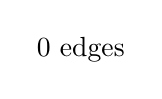
\begin{tikzpicture}
[scale =.35]
\GraphInit[vstyle=Welsh]
\SetGraphUnit{1.6}
\SetVertexNoLabel
\node at (2,-2) { 0 edges};
\Vertex[LabelOut,Lpos=90,x=0,y=0]{$A$}
\Vertex[LabelOut,Lpos= 90,x=2,y=3]{$B$}
\Vertex[LabelOut,Lpos=-90,x=4,y=0]{$C$}
\end{tikzpicture}
\hspace{.5in} %%%%%%%%%%%%%
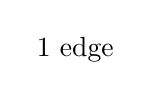
\begin{tikzpicture}
[scale =.35]
\GraphInit[vstyle=Welsh]
\SetGraphUnit{1.6}
\SetVertexNoLabel
\node at (2,-2) {1 edge};
\Vertex[LabelOut,Lpos=90,x=0,y=0]{$A$}
\Vertex[LabelOut,Lpos= 90,x=2,y=3]{$B$}
\Vertex[LabelOut,Lpos=-90,x=4,y=0]{$C$}
\Edges($A$, $B$)
\end{tikzpicture}
\hspace{.5in} %%%%%%%%%%%%%
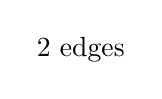
\begin{tikzpicture}
[scale =.35]
\GraphInit[vstyle=Welsh]
\SetGraphUnit{1.6}
\SetVertexNoLabel
\node at (2,-2) {2 edges};
\Vertex[LabelOut,Lpos=90,x=0,y=0]{$A$}
\Vertex[LabelOut,Lpos= 90,x=2,y=3]{$B$}
\Vertex[LabelOut,Lpos=-90,x=4,y=0]{$C$}
\Edges($A$, $B$, $C$)
\end{tikzpicture}
\hspace{.5in} %%%%%%%%%%%%%
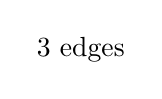
\begin{tikzpicture}
[scale =.35]
\GraphInit[vstyle=Welsh]
\SetGraphUnit{1.6}
\SetVertexNoLabel
\node at (2,-2) {3 edges};
\Vertex[LabelOut,Lpos=90,x=0,y=0]{$A$}
\Vertex[LabelOut,Lpos= 90,x=2,y=3]{$B$}
\Vertex[LabelOut,Lpos=-90,x=4,y=0]{$C$}
\Edges($A$, $B$, $C$, $A$)
\end{tikzpicture}
                \caption{All graphs with three vertices.}
                \label{fig_classify_order3}
            \end{figure}
        \item Classify all graphs with four vertices and three edges.
            \begin{soln}
                There are three such graphs drawn in \Cref{fig_classify_order4_size3}, labeled with their degree sequence. These graphs are not isomorphic because they have different degree sequences. 
            
                To check that this list is complete, suppose that we have a graph with four vertices and three edges.  By \Cref{thm_first_thm_graph_thy}, the sum of the degrees of the vertices is equal to twice the number of edges, which is $2(3)=6$.  The degree sequence must be four nonnegative integers whose sum is equal to six.  We consider the possibilities.
                
                Case 1: The max degree is three.  Notice that every other vertex is adjacent to the degree three vertex, and so the degree sequence is $3,1,1,1$.  We get $K_{1,3}$, which is the graph on the left in \Cref{fig_classify_order4_size3}.

                Case 2: The max degree must be two and there is an isolated vertex.  The degree sequence would have to be $2,2,2,0$.  Moreover, none of the three vertices having degree two can be adjacent to the isolated vertex, so the vertices having degree two must form a 3-cycle, and so we get the graph in the middle in \Cref{fig_classify_order4_size3}.
                
                Case 3: The max degree is two and there is no isolated vertices.  Then, the degree sequence is $2, 2, 1, 1$.  The two degree two vertices must be adjacent to each other, and so we obtain a copy of $P_4$, which is the graph on the right in the graph in the middle of \Cref{fig_classify_order4_size3}.
                
                Notice that checking the graphs were non-isomorphic was much easier than checking that we found all such graphs.
            \end{soln}

            \begin{figure}[hbtp]
                \centering
                %Used in \Cref{sec_graph_ism}.

% K_{1,3}
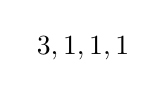
\begin{tikzpicture}
[scale =.35]
\GraphInit[vstyle=Welsh]
\SetGraphUnit{1.6}
\SetVertexNoLabel
\node at (1.5,-2) {$3, 1,1,1$};
\Vertex[LabelOut,Lpos=90,x=0,y=3]{$A$}
\Vertex[LabelOut,Lpos= 90,x=3,y=3]{$B$}
\Vertex[LabelOut,Lpos=-90,x=3,y=0]{$C$}
\Vertex[LabelOut,Lpos=-90,x=0,y=0]{$D$}
\Edges($B$, $A$, $C$)
\Edges($A$, $D$)
\end{tikzpicture}
%%%%%%%%
\hspace{1in} %%%%%%%%
%%%%%%%%
% C_3 \cup K_1
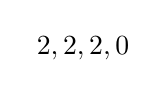
\begin{tikzpicture}
[scale =.35]
\GraphInit[vstyle=Welsh]
\SetGraphUnit{1.6}
\SetVertexNoLabel
\node at (1.5,-2) {$2, 2, 2, 0$};
\Vertex[LabelOut,Lpos=90,x=0,y=3]{$A$}
\Vertex[LabelOut,Lpos= 90,x=3,y=3]{$B$}
\Vertex[LabelOut,Lpos=-90,x=3,y=0]{$C$}
\Vertex[LabelOut,Lpos=-90,x=0,y=0]{$D$}
\Edges($C$, $B$, $D$, $C$)
\end{tikzpicture}
%%%%%%%%
\hspace{1in} %%%%%%%%
%%%%%%%%
% P_4 bent
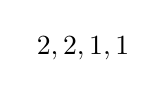
\begin{tikzpicture}
[scale =.35]
\GraphInit[vstyle=Welsh]
\SetGraphUnit{1.6}
\SetVertexNoLabel
\node at (1.5,-2) {$2, 2, 1,1$};
\Vertex[LabelOut,Lpos=90,x=0,y=3]{$A$}
\Vertex[LabelOut,Lpos= 90,x=3,y=3]{$B$}
\Vertex[LabelOut,Lpos=-90,x=3,y=0]{$C$}
\Vertex[LabelOut,Lpos=-90,x=0,y=0]{$D$}
\Edges($D$,$A$, $B$,$C$)
\end{tikzpicture}
                \caption{All graphs with four vertices and three edges.}
                \label{fig_classify_order4_size3}
            \end{figure}
    \end{apart}
\end{exam}

It can be challenging to decide whether a classification is complete.  One tool that can help is graph complements. 

\begin{exam}[Using complements to classify graphs]
\label{exam_using_complements_classify_graphs}
~
    \begin{apart}
        \item \label{part_classify_order4_size2} Classify all graphs with four vertices and two edges.
            \begin{soln}
                If the two edges share a common endpoint, then we get a graph $A$ that has the path $P_3$ and an isolated fourth vertex.  Otherwise, we get a graph $B$ that has two separate copies of $P_2$.  Both are drawn in \Cref{fig_classify_order4_size2_or_size4}. 
            \end{soln}
        \item Use the result of (\ref{part_classify_order4_size2}) to classify all graphs with four vertices and four edges.
            \begin{soln}
                Since the complete graph $K_4$ has six edges, the complement of any graph with four vertices and four edges must have four vertices and two edges. That is, the complement must be one of the two graphs we found in (\ref{part_classify_order4_size2}).  The two graphs with four vertices and four edges are, therefore, $\overline{A}$ and $\overline{B}$ which are also drawn in \Cref{fig_classify_order4_size2_or_size4}. We drew them without edge crossings just for fun, so look closely at the vertex labels.
            \end{soln}
            \begin{figure}[hbtp]
                \centering
                %Used in \Cref{sec_graph_ism}.

\begin{tikzpicture}
[scale =.35]
\GraphInit[vstyle=Welsh]
\SetGraphUnit{1.6}
%\SetVertexNoLabel
\node at (1.5,-2) {$A$};
\Vertex[LabelOut,Lpos=180,x=0,y=3]{$a$}
\Vertex[LabelOut,Lpos= 0,x=3,y=3]{$b$}
\Vertex[LabelOut,Lpos=0,x=3,y=0]{$c$}
\Vertex[LabelOut,Lpos=180,x=0,y=0]{$d$}
\Edges($b$, $c$, $d$)
\end{tikzpicture}
\hspace{.5in} %%%%%%
\begin{tikzpicture}
[scale =.35]
\GraphInit[vstyle=Welsh]
\SetGraphUnit{1.6}
%\SetVertexNoLabel
\node at (0,-2) {$\overline{A}$};
\Vertex[LabelOut,Lpos=180,x=0,y=3]{$a$}
\Vertex[LabelOut,Lpos= 0,x=3,y=3]{$b$}
\Vertex[LabelOut,Lpos=0,x=-2.5,y=5.5]{$c$}
\Vertex[LabelOut,Lpos=180,x=0,y=0]{$d$}
\Edges($a$, $b$, $d$, $a$,$c$)
\end{tikzpicture}
\hspace{.5in} %%%%%
\begin{tikzpicture}
[scale =.35]
\GraphInit[vstyle=Welsh]
\SetGraphUnit{1.6}
%\SetVertexNoLabel
\node at (1.5,-2) {$B$};
\Vertex[LabelOut,Lpos=180,x=0,y=3]{$a$}
\Vertex[LabelOut,Lpos= 0,x=3,y=3]{$b$}
\Vertex[LabelOut,Lpos=0,x=3,y=0]{$c$}
\Vertex[LabelOut,Lpos=180,x=0,y=0]{$d$}
\Edges($a$, $b$)
\Edges($c$, $d$)
\end{tikzpicture}
\hspace{.5in} %%%%%
\begin{tikzpicture}
[scale =.35]
\GraphInit[vstyle=Welsh]
\SetGraphUnit{1.6}
%\SetVertexNoLabel
\node at (1.5,-2) {$\overline{B} $};
\Vertex[LabelOut,Lpos=180,x=0,y=3]{$a$}
\Vertex[LabelOut,Lpos= 0,x=3,y=3]{$c$}
\Vertex[LabelOut,Lpos=0,x=3,y=0]{$b$}
\Vertex[LabelOut,Lpos=180,x=0,y=0]{$d$}
\Edges($a$, $c$, $b$, $d$,$a$)
\end{tikzpicture}

                \caption{All graphs with four vertices and two or four edges.}
                \label{fig_classify_order4_size2_or_size4}
            \end{figure}  
    \end{apart}
\end{exam}
  
Now, it is your turn to try classification.

\begin{act}[Classifying trees]
\label{act_classify_trees}
~
    \begin{actpart}
        \item What is a tree?
        \item Explain why the path $P_3$ is the only tree with three vertices.
        \item There are two trees with four vertices. Draw them.
        \item Classify all trees with five vertices.  That is, make a list of trees having five vertices so that any tree with five vertices is isomorphic to a tree on your list and no two trees on your list are isomorphic.
        \item \label{part_trees_order6} Classify all trees with six vertices. Hint: Organize your work by drawing the longest possible path horizontally.
        \item \label{part_trees_order7} Classify all trees with seven vertices. Hint: Organize your work by drawing the longest possible path horizontally.
    \end{actpart}
\end{act}

%%%%%%%%%%%%%%%%%%%%

\newcommand{\subrobots}{Detour: Robots}
\subsection{\subrobots}
\label{sub_robots}

We continue to practice classification.  
\begin{act}[Robots]
\label{act_robots}
    For the sake of this activity, we invent the following definition.
        \begin{defn}[Robot]
        \label{defn_robot}
            A connected graph is a \textbf{robot} if it contains one 3-cycle and no other cycles.  For example, the graphs drawn in \Cref{fig_robots} are robots.  The left robot has seven vertices, and the right robot has eight.  
                \begin{figure}[hbtp]
                    \centering
                    %Used in \Cref{sec_graph_ism}.

%% Robot 1
\begin{tikzpicture}
    [scale =.3]
    \GraphInit[vstyle=Welsh]
    \SetGraphUnit{1.6}
        \SetVertexNoLabel
    % triangle
    \Vertex[LabelOut,Lpos=90,x=4,y=9]{a}
    \Vertex[
    LabelOut,Lpos=90,x=2,y=6]{b} 
    \Vertex[LabelOut,Lpos=90,x=6,y=6]{c}
    \Edges(a,b,c,a)
    % left leg    
    \Vertex[LabelOut,Lpos=90,x=1,y=3]{d} 
    \Edges(b,d)
    % right legs
    \Vertex[LabelOut,Lpos=90,x=4.5,y=3]{e}
    \Vertex[LabelOut,Lpos=90,x=7.5,y=3]{f} 
    \Vertex[LabelOut,Lpos=90,x=4.5,y=0]{g}
    \Edges(c,e,g)
    \Edges(c,f)
\end{tikzpicture}
%%
\hspace{1in}
% another robot
%%
\begin{tikzpicture}
    [scale =.3]
    \GraphInit[vstyle=Welsh]
    \SetGraphUnit{1.6}
        \SetVertexNoLabel
    % triangle
    \Vertex[LabelOut,Lpos=90,x=2,y=6]{a}
    \Vertex[
    LabelOut,Lpos=90,x=0,y=3]{b} 
    \Vertex[LabelOut,Lpos=90,x=4,y=3]{c}
    \Edges(a,b,c,a)
    % bottom legs    
    \Vertex[LabelOut,Lpos=90,x=0,y=0]{d}
    \Vertex[LabelOut,Lpos=90,x=4,y=0]{e}
    \Edges(b,d)
    \Edges(c,e)
    % headgear
    \Vertex[LabelOut,Lpos=90,x=2,y=9]{f} 
    \Vertex[LabelOut,Lpos=90,x=0,y=12]{g}
    \Vertex[LabelOut,Lpos=90,x=4,y=12]{h}
    \Edges(a,f)
    \Edges(g,f,h)
\end{tikzpicture}
                    \caption{Two robots.}
                    \label{fig_robots}
                \end{figure}
        \end{defn}
    \begin{actpart}
        \item The only robot with three vertices is a 3-cycle.  There is only one robot with four vertices.  Draw it and explain why it is the only one.
        \item There are three different robots with five vertices.  Draw them.
        \item How many different robots are there with six vertices. Hint: Organize your work based on how many vertices of the 3-cycle have edges beyond the 3-cycle -- all three, two of them, or only one of them.
    \end{actpart}
\end{act}

%%%%%%%%%%%%%%%%%%%%%%%%%%%%%%%%%%%%%%%%

\subsection{Exercises}

%%%%%%%%%%%%%%%%%%%%%%%%%%%%%%%%%%%%%%%%

\subsubsection*{Exercises for \Cref{sub_nonisomorphic_graphs}
\subnonisograph}

\begin{exer}[\exerP] % show graphs in a 5-cycle are nonisomorphic]
\label{exer_show_nonism_Ham5}
    Show that the graphs drawn in \Cref{fig_nonism_Ham5} are nonisomorphic by finding a graph invariant that distinguishes the two graphs.
        \begin{figure}[hbtp]
            \centering
            %Used in \Cref{sec_graph_ism}.


\begin{tikzpicture}
[scale =.45]
\GraphInit[vstyle=Welsh]
\SetGraphUnit{1.6}
\SetVertexNoLabel
\Vertex[LabelOut,Lpos=90,x=.6,y=3]{$A$}
\Vertex[LabelOut,Lpos= 90,x=2.4,y=3]{$B$}
\Vertex[LabelOut,Lpos=-90,x=3,y=1.2]{$C$}
\Vertex[LabelOut,Lpos= -90,x=1.5,y=0]{$D$}
\Vertex[LabelOut,Lpos= -90,x=0,y=1.2]{$E$}
\Edges($A$, $B$, $C$, $D$, $E$, $A$)
\Edges($A$,$D$,$B$)
\Edges($C$,$E$)
\end{tikzpicture}
\hspace{1in} %%%%%

\begin{tikzpicture}
[scale =.45]
\GraphInit[vstyle=Welsh]
\SetGraphUnit{1.6}
\SetVertexNoLabel
\Vertex[LabelOut,Lpos=90,x=.6,y=3]{$A$}
\Vertex[LabelOut,Lpos= 90,x=2.4,y=3]{$B$}
\Vertex[LabelOut,Lpos=-90,x=3,y=1.2]{$C$}
\Vertex[LabelOut,Lpos= -90,x=1.5,y=0]{$D$}
\Vertex[LabelOut,Lpos= -90,x=0,y=1.2]{$E$}
\Edges($A$, $B$, $C$, $D$, $E$, $A$)
\Edges($B$,$E$,$C$)
\Edges($C$,$A$)
\end{tikzpicture}
            \caption{Nonisomorphic graphs for \Cref{exer_show_nonism_Ham5}.}
                \label{fig_nonism_Ham5}
        \end{figure}
\end{exer}

\begin{exer}[\exerP] %  use complement to show nonisomorphic]
\label{exer_show_nonism_H3b6}
    Use complements to show that the graphs drawn in \Cref{fig_nonism_H3b6} are nonisomorphic by finding a graph invariant that distinguishes the complements of the two graphs.
        \begin{figure}[hbtp]
            \centering
            % Used in \Cref{sec_graph_ism}.

\begin{tikzpicture}
[scale =.5]
\GraphInit[vstyle=Welsh]
\SetGraphUnit{1.6}
\SetVertexNoLabel
\Vertices{circle}{$a$,$b$,$c$,$d$,$e$,$r$}
\Edges($a$, $b$, $c$, $d$, $e$,$r$,$a$)
\Edges($c$,$r$)
\Edges($b$,$e$)
\Edges($a$,$d$)
\end{tikzpicture}
\hspace{1in}%%%%%
% \begin{tikzpicture}
% [scale=.85,auto=left,every node/.style={circle,draw=black, fill=white, inner sep=.06in}]
% \def \n {6}
% \def \radius {1cm}
% \def \margin {6} % margin in angles, depends on the radius
% \foreach \s in {1,...,\n}
% {
%   \node(\s) at ({360/\n * (\s - 1)}:\radius) {};
% }
% \draw[thick] (1) to (2) to (3) to (4) to (5) to (6) to (1);
% \draw[thick] (1) to (4); 
% \draw[thick] (2) to (6);
% \draw[thick] (3) to (5);
% \end{tikzpicture}
\begin{tikzpicture}
[scale =.5]
\GraphInit[vstyle=Welsh]
\SetGraphUnit{1.6}
\SetVertexNoLabel
\Vertices{circle}{$a$,$b$,$c$,$d$,$e$,$r$}
\Edges($a$, $b$, $c$, $d$, $e$,$r$,$a$)
\Edges($b$,$r$)
\Edges($c$,$e$)
\Edges($a$,$d$)
\end{tikzpicture}
            \caption{Nonisomorphic graphs for \Cref{exer_show_nonism_H3b6}.}
                \label{fig_nonism_H3b6}
        \end{figure}
\end{exer}

\begin{exer}[\exerP] %  decide if $H_{3,6}$ and $K_{3,3}$ are isomorphic]
\label{exer_show_ism_H3b6_K3b3}
    Decide whether the graphs in \Cref{fig_ism_H3b6_K3b3} are isomorphic and carefully justify your answer.
        \begin{figure}[hbtp]
            \centering
            %Used in \Cref{sec_graph_ism}.

\begin{tikzpicture}
[scale =.5]
\GraphInit[vstyle=Welsh]
\SetGraphUnit{1.6}
\SetVertexNoLabel
\Vertices{circle}{$a$,$b$,$c$,$d$,$e$,$r$}
\Edges($a$, $b$, $c$, $d$, $e$,$r$,$a$)
\Edges($c$,$r$)
\Edges($b$,$e$)
\Edges($a$,$d$)
\end{tikzpicture}
\hspace{1 in} %%%%%
\begin{tikzpicture}
[scale =.35]
\GraphInit[vstyle=Welsh]
\SetGraphUnit{1.6}
\SetVertexNoLabel
\Vertex[LabelOut,Lpos=90,x=0,y=3]{$a$}
\Vertex[LabelOut,Lpos= 90,x=0,y=0]{$b$}
\Vertex[LabelOut,Lpos= 90,x=3,y=3]{$c$}
\Vertex[LabelOut,Lpos= 90,x=3,y=0]{$d$}
\Vertex[LabelOut,Lpos= 90,x=6,y=3]{$e$}
\Vertex[LabelOut,Lpos= 90,x=6,y=0]{$r$}
\Edges($a$, $b$, $c$, $d$, $e$,$r$,$a$)
\Edges($c$,$r$)
\Edges($b$,$e$)
\Edges($a$,$d$)
\end{tikzpicture}

            \caption{The Harary graph $H_{3,6}$ and the complete bipartite graph $K_{3,3}$ for \Cref{exer_show_ism_H3b6_K3b3}.}
            \label{fig_ism_H3b6_K3b3}
        \end{figure}    
\end{exer}

\begin{exer}[\exerP] %  decide if order 5 graphs are isomorphic]
\label{exer_show_nonism_order5}
    Decide whether the graphs in \Cref{fig_nonism_order5} are isomorphic and carefully justify your answer.
        \begin{figure}[hbtp]
            \centering
            %Used in \Cref{sec_graph_ism}.


\begin{tikzpicture}
[scale =.45]
\GraphInit[vstyle=Welsh]
\SetGraphUnit{1.6}
\SetVertexNoLabel
\Vertex[LabelOut,Lpos=90,x=0,y=3]{$A$}
\Vertex[LabelOut,Lpos= 90,x=3,y=3]{$B$}
\Vertex[LabelOut,Lpos=-90,x=3,y=0]{$C$}
\Vertex[LabelOut,Lpos=-90,x=0,y=0]{$D$}
\Vertex[LabelOut,Lpos=-90,x=1.5,y=1.5]{$X$}
\Edges($A$, $B$, $C$, $D$, $A$)
\Edges($A$,$X$, $C$)
\Edges($D$,$X$)
\end{tikzpicture}
\hspace{1in} %%%%%

\begin{tikzpicture}
[scale =.5]
\GraphInit[vstyle=Welsh]
\SetGraphUnit{1.6}
\SetVertexNoLabel
\Vertex[LabelOut,Lpos=90,x=.6,y=3]{$A$}
\Vertex[LabelOut,Lpos= 90,x=2.4,y=3]{$B$}
\Vertex[LabelOut,Lpos=-90,x=3,y=1.2]{$C$}
\Vertex[LabelOut,Lpos= -90,x=1.5,y=0]{$D$}
\Vertex[LabelOut,Lpos= -90,x=0,y=1.2]{$X$}
\Edges($A$, $B$, $C$, $D$, $A$)
\Edges($A$,$X$, $C$)
\Edges($D$,$X$)
\end{tikzpicture}
            \caption{The graphs for \Cref{exer_show_nonism_order5}.}
            \label{fig_nonism_order5}
        \end{figure}    
\end{exer}

\begin{exer}[\exerP] %  use complement to decide if order 4 graphs are isomorphic]
\label{exer_show_ism_K4_minus_edge}
    Use complements to decide whether the graphs in \Cref{fig_ism_K4_minus_edge} are isomorphic and carefully justify your answer.
        \begin{figure}[hbtp]
            \centering
            %Used in \Cref{sec_graph_ism}.

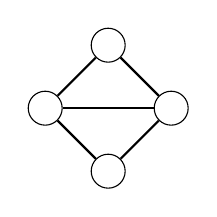
\begin{tikzpicture}
[scale=.8,auto=left,every node/.style={circle,draw=black, fill=white, inner sep=.06in}]
\def \n {4}
\def \radius {1cm}
\def \margin {4} % margin in angles, depends on the radius
\foreach \s in {1,...,\n}
{
  \node(\s) at ({360/\n * (\s - 1)}:\radius) {};
}
\draw[thick] (1) to (2) to (3) to (4)  to (1);
\draw[thick] (1) to (3); 
\end{tikzpicture}
\hspace{1in} %%%%%
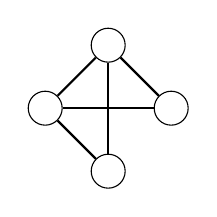
\begin{tikzpicture}
[scale=.8,auto=left,every node/.style={circle,draw=black, fill=white, inner sep=.06in}]
\def \n {4}
\def \radius {1cm}
\def \margin {4} % margin in angles, depends on the radius
\foreach \s in {1,...,\n}
{
  \node(\s) at ({360/\n * (\s - 1)}:\radius) {};
}
\draw[thick] (1) to (2) to (3) to (4) ;
\draw[thick] (1) to (3) ;
\draw[thick] (2) to (4) ;
\end{tikzpicture}
            \caption{The graphs for \Cref{exer_show_ism_K4_minus_edge}.}
            \label{fig_ism_K4_minus_edge}
        \end{figure}    
\end{exer}

\begin{exer}[\exerU] %  decide if order 6 graph are isomorphic]
\label{exer_show_nonism_order6}
    Decide whether the graphs in \Cref{fig_nonism_order6} are isomorphic and carefully justify your answer.
        \begin{figure}[hbtp]
            \centering
            %Used in \Cref{sec_graph_ism}.

\begin{tikzpicture}
[scale =.25]
\GraphInit[vstyle=Welsh]
\SetGraphUnit{1.6}
\SetVertexNoLabel
\Vertex[LabelOut,Lpos=90,x=0,y=2]{$a$}
\Vertex[LabelOut,Lpos= 90,x=0,y=5]{$b$}
\Vertex[LabelOut,Lpos= 90,x=3,y=7]{$c$}
\Vertex[LabelOut,Lpos= 90,x=6,y=5]{$d$}
\Vertex[LabelOut,Lpos= 90,x=6,y=2]{$e$}
\Vertex[LabelOut,Lpos= 90,x=3,y=0]{$r$}
\Edges($a$, $b$, $c$, $d$, $e$,$r$,$a$)
\Edges($c$,$r$)
\end{tikzpicture}
\hspace{1in} %%%%%
\begin{tikzpicture}
[scale =.25]
\GraphInit[vstyle=Welsh]
\SetGraphUnit{1.6}
\SetVertexNoLabel
\Vertex[LabelOut,Lpos=90,x=0,y=2]{$a$}
\Vertex[LabelOut,Lpos= 90,x=0,y=5]{$b$}
\Vertex[LabelOut,Lpos= 90,x=3,y=7]{$c$}
\Vertex[LabelOut,Lpos= 90,x=6,y=5]{$d$}
\Vertex[LabelOut,Lpos= 90,x=6,y=2]{$e$}
\Vertex[LabelOut,Lpos= 90,x=3,y=0]{$r$}
\Edges($a$, $b$, $c$, $d$, $e$,$r$,$a$)
\Edges($c$,$a$)
\end{tikzpicture}
            \caption{The graphs for \Cref{exer_show_nonism_order6}.}
            \label{fig_nonism_order6}
        \end{figure}    
\end{exer}

\begin{exer}[\exerU] %  use complement to decide if order complicated graphs are isomorphic]
\label{exer_show_nonism_complicated_Ham8}
    Use complements to decide whether the graphs in \Cref{fig_nonism_complicated_Ham8} are isomorphic and carefully justify your answer.
        \begin{figure}[hbtp]
            \centering
            %Used in \Cref{sec_graph_ism}.
 
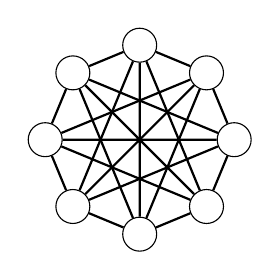
\begin{tikzpicture}
[scale=1.2,auto=left,every node/.style={circle,draw=black, fill=white, inner sep=.06in}]
\def \n {8}
\def \radius {1cm}
\def \margin {8} % margin in angles, depends on the radius
\foreach \s in {1,...,\n}
{
  \node(\s) at ({360/\n * (\s - 1)}:\radius) {};
}
\draw[thick] (1) to (2) to (3) to (4) to (5) to (6) to (7) to (8) to (1);
\draw[thick] (1) to (4) to (8) to (5) to (1); 
\draw[thick] (2) to (6) to (3) to (7) to (2); 
\draw[thick] (1) to (6);
\draw[thick] (2) to (5);
\draw[thick] (3) to (8);
\draw[thick] (4) to (7);
\end{tikzpicture}
\hspace{1in} %%%%%
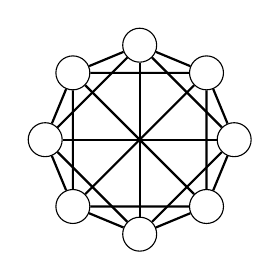
\begin{tikzpicture}
[scale=1.2,auto=left,every node/.style={circle,draw=black, fill=white, inner sep=.06in}]
\def \n {8}
\def \radius {1cm}
\def \margin {8} % margin in angles, depends on the radius
\foreach \s in {1,...,\n}
{
  \node(\s) at ({360/\n * (\s - 1)}:\radius) {};
}
\draw[thick] (1) to (2) to (3) to (4) to (5) to (6) to (7) to (8) to (1);
\draw[thick] (1) to (5) ;
\draw[thick] (2) to (6) ;
\draw[thick] (3) to (7) ;
\draw[thick] (4) to (8) ;
\draw[thick] (1) to (3) to (5) to (7) to (1);
\draw[thick] (2) to (4) to (6) to (8) to (2);
\end{tikzpicture}
            \caption{The graphs for \Cref{exer_show_nonism_complicated_Ham8}.}
            \label{fig_nonism_complicated_Ham8}
        \end{figure}    
\end{exer}

\begin{exer}[\exerR] % nonisomorphic
\label{exer_dyk_nonism}
    Do you know \ldots
        \begin{exerpart}
            \item What a graph invariant is?
            \item Why finding a distinguishing invariant proves that two graphs are not isomorphic?
            \item What some examples of graph invariants are?
            \item How we can prove that two graphs are not isomorphic (by finding a distinguishing invariant)?
            \item How to use complements to prove that two graphs are isomorphic or nonisomorphic?
            \item How to use planarity-style moves to decide whether two graphs are isomorphic or not? 
        \end{exerpart}
\end{exer}

\begin{exer}[\exerE] %  decide if order 7 graphs are isomorphic]
\label{exer_show_nonism_order7}
    Decide whether the graphs in \Cref{fig_nonism_order7} are isomorphic and carefully justify your answer.
        \begin{figure}[hbtp]
            \centering
            %Used in \Cref{sec_graph_ism}.

\begin{tikzpicture}
[scale =.2]
\GraphInit[vstyle=Welsh]
\SetGraphUnit{1.6}
\SetVertexNoLabel
\Vertex[LabelOut,Lpos=-90,x=0,y=-3]{$a$}
\Vertex[LabelOut,Lpos= -90,x=3,y=0]{$b$}
\Vertex[LabelOut,Lpos= -90,x=7,y=0]{$e$}
\Vertex[LabelOut,Lpos= -90,x=10,y=-3]{$f$}
\Vertex[LabelOut,Lpos=90,x=0,y=7]{$1$}
\Vertex[LabelOut,Lpos= 90,x=5,y=4]{$3$}
\Vertex[LabelOut,Lpos= 90,x=10,y=7]{$6$}
\Edges($a$, $b$, $e$,$f$)
\Edges($1$, $6$, $f$, $a$, $1$)
\Edges($1$,$3$,$6$)
\Edges($b$,$3$,$e$)
\end{tikzpicture}
\hspace{1in} %%%%%
\begin{tikzpicture}
[scale =.2]
\GraphInit[vstyle=Welsh]
\SetGraphUnit{1.6}
\SetVertexNoLabel
\Vertex[LabelOut,Lpos=-90,x=0,y=-3]{$a$}
\Vertex[LabelOut,Lpos= -90,x=3,y=0]{$b$}
\Vertex[LabelOut,Lpos= -90,x=7,y=0]{$e$}
\Vertex[LabelOut,Lpos= -90,x=10,y=-3]{$f$}
\Vertex[LabelOut,Lpos=90,x=0,y=7]{$1$}
\Vertex[LabelOut,Lpos= 90,x=5,y=4]{$3$}
\Vertex[LabelOut,Lpos= 90,x=10,y=7]{$6$}
\Edges($a$, $b$, $e$,$f$)
\Edges($1$, $6$, $f$, $a$, $1$)
\Edges($3$,$6$)
\Edges($b$,$3$,$e$)
\Edges($1$,$e$)
\end{tikzpicture}

            \caption{The graphs for \Cref{exer_show_nonism_order7}.}
            \label{fig_nonism_order7}
        \end{figure}    
\end{exer}

%%%%%%%%%%%%%%%%%%%%%%%%

\subsubsection*{Exercises for \Cref{sub_graph_classification}
\subgraphclassification}

In these classification exercises, no justification is required, but make sure that your list is complete and that no two graphs on your list are isomorphic.

\begin{exer}[\exerP] %  classify all graphs that are 8-cycle plus an edge]
\label{exer_classify_8cycle_plus_edge}
    Classify all graphs with eight vertices and nine edges that contain an 8-cycle. 
\end{exer}

\begin{exer}[\exerU] %  classify all graphs with 4 vertices]
\label{exer_classify_order4}
    Classify all graphs with four vertices. Hint: \Cref{exam_classify_order3_order4} and
    \Cref{exam_using_complements_classify_graphs} are useful.
\end{exer}

\begin{exer}[\exerU] %  classify all graphs with 5 vertices]
\label{exer_classify_order5}
    Classify all connected graphs with five vertices and six edges.
\end{exer}

\begin{exer}[\exerU] %  classify all trees with 6 or 7 vertices]
\label{exer_classify_trees_order6_order7}
~
    \begin{exerpart}
        \item Classify all trees with six vertices.  Yes, this exercise repeats \Cref{act_classify_trees} (\ref{part_trees_order6}). Hint: organize your work by drawing the longest possible path horizontally.
        \item Classify all trees with seven vertices.  Yes, this exercise repeats \Cref{act_classify_trees} (\ref{part_trees_order7}). Hint: organize your work by drawing the longest possible path horizontally.
    \end{exerpart}
\end{exer}

\begin{exer}[\exerR] % classify graphs
\label{exer_dyk_classify_graphs}
    Do you know \ldots
        \begin{exerpart}
            \item What we mean by classifying graphs of a certain type?
            \item How to use complements to help classify graphs?
            \item How to organize your work when classifying graphs? (There are several ways.) 
        \end{exerpart}
\end{exer}

\begin{exer}[\exerE] %  classify all regular graphs with 6 vertices]
\label{exer_classify_regular}
    Classify all regular graphs with six vertices.  Recall that in a regular graph, all vertices have the same degree $r$.  Consider the cases $r=0$, $r=1$, $r=2$, $r=3$, $r=4$, and $r=5$.
\end{exer}

\begin{exer}[\exerE] %  classify all trees with 8 vertices]
\label{exer_classify_trees_order8}
    Classify all trees with eight vertices. Hint: Organize your work by drawing the longest possible path horizontally. Another hint: there are 23 of them. 
\end{exer}

%%%%%%%%%%%%%%%%%%%%%%%%
\subsection*{Exercises for \Cref{sub_robots} \subrobots}

\begin{exer}[\exerP] %  super robots]
\label{exer_super_robot}
    A connected graph is \vocab{super-robot} if it contains one 4-cycle and no other cycles.  Draw a super-robot with six vertices, one with seven vertices, and one with eight vertices.
\end{exer}

\begin{exer}[\exerE] %  robots with seven vertices]
\label{exer_robots7}
    Classify all robots with seven vertices. No justification is required, but make sure that your list is complete and that no two robots on your list are isomorphic.
\end{exer}

\begin{exer}[\exerE] %  all super robots with eight vertices]
\label{exer_super_robot8}
    Super-robots were defined in \Cref{exer_super_robot}. Draw all super-robots with eight vertices. No justification is required, but make sure that your list is complete and that no two super-robots on your list are isomorphic.
\end{exer}

%%%%%%%%%%%%%%%%%%%%%%%%%%%
\subsection{\answers}
%%%%%%%%%%%%%%%%%%%%%%%%%%%

\subsubsection{\answers for \Cref{sub_nonisomorphic_graphs} \subnonisograph}

\subsubsection*{\Cref{exer_show_nonism_Ham5} \answers}
    Hint:  One answer is that the graph on the left has the degree sequence $4,3,3,3,3$, but the graph on the right has a different degree sequence.  Can you find an easier answer?

\subsubsection*{\Cref{exer_show_nonism_H3b6} \answers}
    The complement of the graph on the left is disconnected (it is two copies of $C_3$), but the graph on the right has a complement that is connected (it is isomorphic to $C_6$).

\subsubsection*{\Cref{exer_show_ism_H3b6_K3b3} \answers}
    Hint: They are isomorphic.  To prove that they are isomorphic, label the vertices so that they have the same vertices and the same edges.  (It is not enough to show that they have many invariants in common.)

\subsubsection*{\Cref{exer_show_nonism_order5} \answers}
    Hint: They are isomorphic.  Label the vertices so that they have the same vertices and the same edges.  Start with the degree two vertices, then their neighbors.

\subsubsection*{\Cref{exer_show_ism_K4_minus_edge} \answers}
    Hint: They are isomorphic. Their complements are a copy of $P_2$ and two isolated vertices.  Prove that the complements are isomorphic by labeling the vertices.

\subsubsection*{\Cref{exer_show_nonism_order6} \answers}
    Hint: They are not isomorphic.  You can find a distinguishing invariant based on the cyclic subgraphs.  

\subsubsection*{\Cref{exer_show_nonism_complicated_Ham8} \answers}
    Hint: Look closely at the complements.  The complements are nonisomorphic.  Explain why.

\subsubsection*{\Cref{exer_show_nonism_order7} \answers}
    Hint: Look at the neighbors of the degree four vertex.  How are they adjacent to one another?

%%%%%%%%%%%%

\subsubsection{\answers for \Cref{sub_graph_classification}
\subgraphclassification}

\subsubsection*{\Cref{exer_classify_order4} \answers}
    Hint: There are 11 total. One graph has no edges, and one graph has one edge. \Cref{exam_using_complements_classify_graphs} lists all graphs with two edges and four edges.  \Cref{exam_classify_order3_order4} lists the graphs with three edges.  The graphs with five or six edges are the complements of graphs already on the list.

\subsubsection*{\Cref{exer_classify_order5} \answers}
    Hint: Small graphs are often given names that describe what they look like.  Four of the answers are named the house, the kite, the dart, and the bowtie.  (Please figure these out yourself, without peeking at resources!) There is one more possibility, but I do not know if it has a name.

\subsubsection*{\Cref{exer_classify_trees_order6_order7} \answers}
    \begin{apart}
        \item Hint: There are six.
        \item Hint: There are 11.
    \end{apart}

\subsubsection*{\Cref{exer_classify_regular} \answers}
    Hint: There are one 0-regular, one 1-regular, and two 2-regular graphs.  You can check if you have the correct number of 3-regular, 4-regular, and 5-regular by considering their complements.

%%%%%%%%%%%%
\subsubsection{\answers for \Cref{sub_robots} \subrobots}

None provided.
%%%%%%%%%%%%
